\section{Basics of \gls{lidar}}
\label{sec:chap_lidar_basics}

\gls{lidar} is a technology based on laser time of flight to measure distances. \citet{lidar_basics} present the physical details as well as the pros and cons of three time of flight commonly used in \gls{lidar}s, namely the pulsed, phase-shift and frequency modulated continuous wave. In the context of our research, we focus more on higher level concepts that could cause sensor readings to be erroneous for modeling 3D environments or objects. Beams emitted by a \gls{lidar} have a given with width and angle at source. This cause the beam two-dimensional pattern on the target to grow with distance. Once the light hit the target, it bounces back to the sensor which will extract the range information out of it. Obviously, when the target material is highly absorbent or reflective, the light might not reach back the sensor. Otherwise, the sensor will receive the signal which may be represented by a curve of light intensity as function of time. Smooth lambertian surfaces will produce a unimodal distribution with which it is easy to calculate the target range, but multi-modal waveforms caused by partially transparent material, fog, dust, small objects and edges lead to an ambiguous interpretation. Figure~\ref{fig:lidar_basics} depict laser beam hitting different targets along with the resulting waveforms. While some \gls{lidar}s provide full waveform, they generally only output a single or few echoes and the inference method differs from sensor to sensor (e.g., using the first or last maximum, using the mean). For this reason, it is important to determine whether the sensor of your choice is well suited to your needs. Figure~\ref{fig:shadow_points} show how reading errors affect the 3D representation of the environment surrounding the robot. \todo{Rephrase} Note that it is possible to obtain a complete 3D representation as shown in Figure through a pivoting internal mirror to the sensor and / or an external motor rotating the sensor.

\begin{figure}[htpb]
    \centering
    \subfloat[test]{\label{fig:a}}{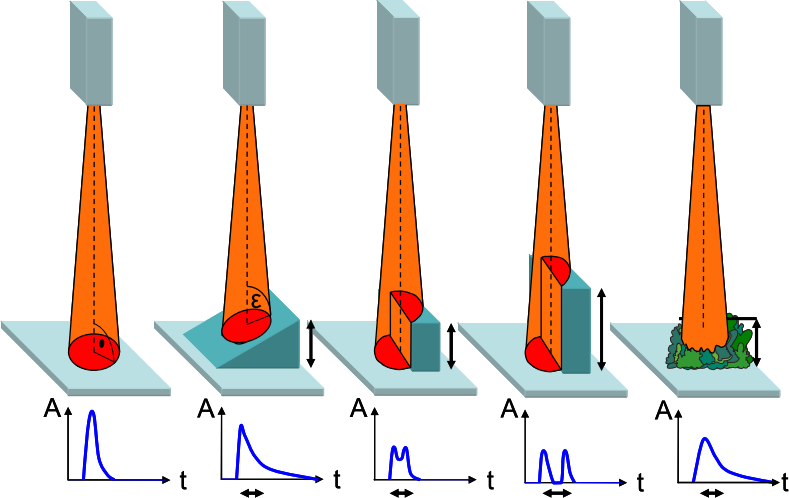
\includegraphics[width=0.8\linewidth]{img/chap_lidar/waveforms.png}}\\\vspace{1em}
    \subfloat{\label{fig:b}}{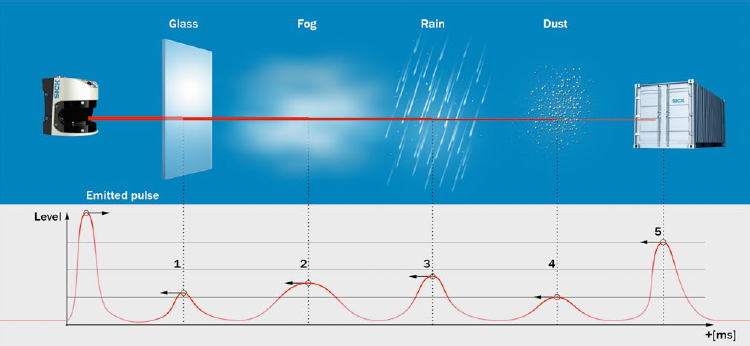
\includegraphics[width=0.8\linewidth]{img/chap_lidar/waveforms2.png}}
    \caption{A representation of \gls{lidar} beams hitting different structures along with the resulting waveforms.  From \citet{lidar_figure1}. Yo dang (http://www.robotsinsearch.com/products/lms500-21000-lite) \todo{Write some caption and add the SICK ref}}
    \label{fig:lidar_basics}
\end{figure}

\begin{figure}[htpb]
    \centering
    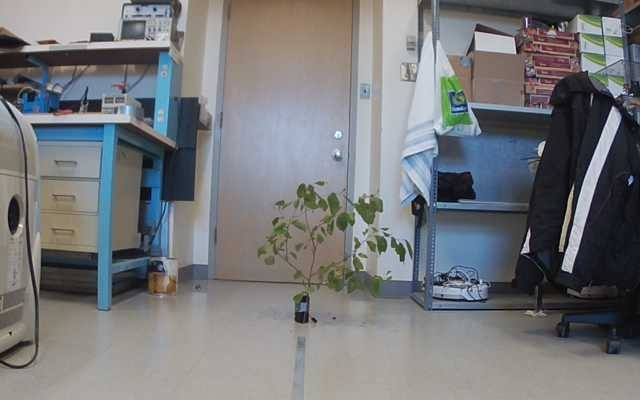
\includegraphics[width=0.9\linewidth]{img/chap_lidar/shadow_image.jpg}\\\vspace{1em}
    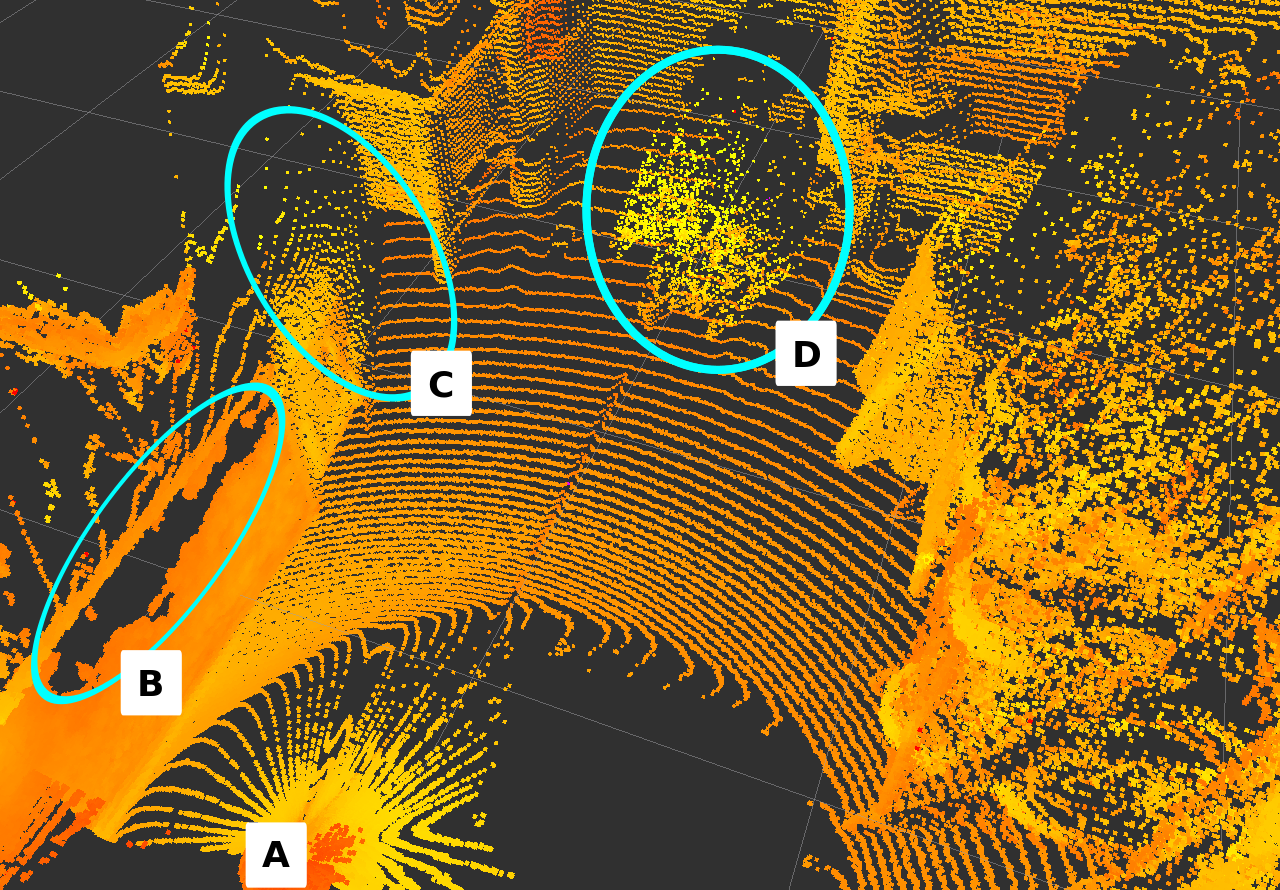
\includegraphics[width=0.9\linewidth]{img/chap_lidar/shadow_pointcloud.png}
    \caption{A picture of a scene (top) and a diagonal view of the point cloud (bottom) resulting from the acquisition by the SICK LMS151 \gls{lidar} mounted on a pan and tilt unit. The sensor position is represented by \textbf{A}. Region \textbf{B} shows missing points caused by absorbent material (a black box not visible in the picture). Region \textbf{C} shows noisy points caused by the edge of an object while region \textbf{D} shows a particularly bad \gls{3d} representation of a fine structure (tree branch).}
    \label{fig:shadow_points}
\end{figure}
